% ---------------------------------------------------------------------------
% Section 5.6: neural judges and sample sets at scale.
% Every number below is in results/jmlr/samples/: judge_numbers.json, analysis_claude.json,
% claude_extra.json, claude_curve.json, analysis_opus.json (frontier generator),
% gpt5_extra.json and analysis_gpt5.json (GPT-5 judge), samples_fmnist.json.
% ---------------------------------------------------------------------------
\subsection{Neural judges and sample sets at scale}
\label{sec:exp-judge}

Some of the most expensive comparisons in current practice are made by
neural judges. Language models are widely used to judge pairs of outputs
\citep{zheng2023judging}; here a judge reads two outputs and scores how
different they are, as natural-language-inference and equivalence judges do
in diversity benchmarks \citep{stasaski2022semantic,zhang2025noveltybench}. Such a judge has no feature map, so the
all-pairs average costs at least one judge call per pair. Its scores also
need not satisfy the triangle inequality, so \Cref{thm:metric} need not
apply (although the Claude table at $T=1$ below violates none of its
$124{,}992$ triangle inequalities).
\Cref{thm:balanced}, \Cref{cor:efficiency},
\Cref{prop:sparse-anatomy,prop:rr-variance}, and the Horvitz--Thompson variance of \Cref{rem:ht-variance} do apply, because
they hold for every table, and every judge table below is symmetric by
construction. We sampled populations of $n=300$ responses from
\mbox{Qwen2.5-0.5B-Instruct} \citep{qwen2024qwen25} and
\mbox{Llama-3.2-1B-Instruct} \citep{grattafiori2024llama}. Each of $18$
populations answers one of three open-ended prompts (a one-sentence story about a robot, a name for a new coffee shop, and one sentence of advice for a first job) at temperature $T=0.5$,
$1$, or $1.5$, and three further populations mix prompts, mix generators,
or plant $2\%$ degenerate samples. Three more contain $300$ responses each
from Claude~Opus~5.5 to the same prompts, with default sampling (the API no
longer accepts a sampling temperature). A cross-encoder trained for semantic
textual similarity \citep[STS;][]{reimers2019sentence,cer2017semeval} scored every
pair in both orders, giving $d_{ij}=1-\bar s_{ij}$ with $\bar s_{ij}\in[0,1]$
the mean of the two scores. That is $89{,}700$ judge calls and $48$--$98$
GPU-seconds per population. For the first $64$ Qwen story responses at
$T=0.5$ and at $T=1$, Claude~Opus~5.5 (Anthropic) also rated all $2{,}016$
pairs from $0$ to $10$, giving $d_{ij}$ as the rating divided by $10$
(\Cref{app:exp-details:judge}).

\begin{figure}[t]
  \centering
  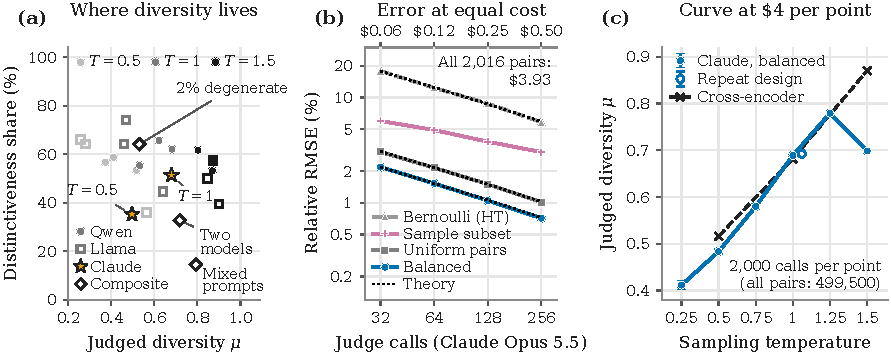
\includegraphics[width=\textwidth]{figures/fig_judge.pdf}
  \caption{\textbf{Generated text scored by neural judges.}
  (a) Judged diversity $\mu$ and the share of the pairwise variance carried
  by distinctiveness. There are $21$ cross-encoder tables with $n=300$:
  Qwen (filled circles) and Llama (open squares), shaded by sampling
  temperature, and three composite populations (diamonds). The stars are
  the first $64$ Qwen story responses at $T=0.5$ and $T=1$, judged by
  Claude~Opus~5.5 instead of the cross-encoder. (b) Relative RMSE
  against the number of Claude calls for the $64$ Qwen story responses at
  $T=1$. Colored lines and markers are measured over $4{,}000$ draws. Black
  dotted lines are the closed-form standard deviations of \Cref{thm:balanced}
  and \Cref{cor:efficiency}, and the square root of the Horvitz--Thompson
  variance of \Cref{rem:ht-variance}; the closed form of \Cref{thm:general-design} for the sample subset
  is not drawn.
  The top axis gives the API cost. (c) A diversity curve at linear cost:
  Claude-judged diversity of $1{,}000$ \mbox{Qwen2.5-0.5B-Instruct} story responses
  per temperature, each point from one randomized round-robin design with
  $k=4$ rounds ($2{,}000$ calls, about \$4; all pairs would take $499{,}500$),
  with the design-based $95\%$ interval of \Cref{prop:rr-variance} ($t$ with
  $3$ degrees of freedom), conditional on the $1{,}000$ sampled responses; except
  at $T=0.25$ the intervals are narrower than the markers. The
  open marker (offset for legibility) is an independent second design on the
  same responses. Dashed black: the exact all-pairs
  cross-encoder diversity of separate $300$-response samples from the same
  generator and prompt (another scale and sample: compare shapes).}
  \label{fig:judge}
\end{figure}

\paragraph{Where judged diversity lives.} Judged diversity rises with
temperature: for Qwen, $\mu$ ranges over $0.37$--$0.52$ at $T=0.5$ and
$0.80$--$0.87$ at $T=1.5$. Its anatomy, however, shows no consistent trend
with temperature. For a single prompt and a small generator scored by the cross-encoder,
distinctiveness carries $36$--$74\%$
of the pairwise variance (\Cref{fig:judge}(a)), because individual samples
differ in how far they sit from all others, and the anatomy names them. At
$T=0.5$, the three least distinctive of the $300$ samples under the
cross-encoder are variants of one template (``A sleek humanoid robot named
Echo\ldots''), and two of the three least distinctive of the $64$ under
Claude are Echo variants as well. At $T=1$, the two most distinctive samples under Claude are a
response that switched to Chinese and an off-topic hacker story. Under the
cross-encoder, on the same $64$ responses, the hacker story ranks first and
the Chinese response third; on all $300$, a ``Lorem ipsum'' passage also
enters the top three. Planting six degenerate samples among $300$ raises the
distinctiveness share from $53\%$ to $64\%$. Mixing the three prompts at
$T=1$ lowers it from $55$--$66\%$ to $15\%$, because the prompts act as
roles and the structure becomes relational.

\paragraph{Frontier models as generators and as judges.} Responses from a
frontier model are far less diverse under this judge, as other measures
also find \citep{zhang2025noveltybench,jiang2025hivemind}. (The contrast is
descriptive: the open models were capped at $40$ new tokens, so $66$--$100\%$ of
their responses end mid-sentence, whereas the API model's are complete.) For the Claude~Opus~5.5 populations, $\mu$ is
only $0.22$--$0.41$, below every Qwen population at $T=1$
($0.53$--$0.68$). The anatomy separates coffee-shop names that fall into a
few modes ($17\%$ distinctiveness, so mostly relational) from advice that
repeats one template with idiosyncratic exceptions ($69\%$). The closed
forms hold here as well; for example, the story prompt at $m=2n$ gives
$0.89\%$ error against $0.89\%$ predicted, and single-design intervals cover
$\mu$ in $94.6$--$95.9\%$ of draws. Claude and the cross-encoder score on different scales (a rating divided
by $10$ against one minus an STS probability), so we compare them by rank:
they correlate $0.54$--$0.68$ pair by pair, and their distinctiveness
rankings of the $64$ responses have Spearman correlations of $0.53$ ($T=1$)
and $0.80$ ($T=0.5$). A third judge from another vendor, GPT-5 (OpenAI),
scored the same $2{,}016$ pairs at $T=1$. It gives $\mu=0.682$, correlates
$0.64$ with Claude pair by pair (Claude's own order-swapped retest gives
$0.74$), and ranks the $64$ responses by distinctiveness with a Spearman
correlation of $0.86$ against Claude, with the same two responses on top.
The closed forms hold on its table too ($0.89\%$ error at $m=2n$ against
$0.90\%$ predicted).

\paragraph{Fewer judge calls, with error bars.} Here the estimand is
the diversity of the sampled responses, and errors refer to the design;
claims about a generator add the sampling variance $4\zeta_1/n+O(n^{-2})$
(\Cref{sec:discussion}). Claude's order-swapped retest puts call noise at up
to $46\%$ of $\sigmaint$ ($T=1$), and $97\%$ of such noise is relational, so
$\kappa=1.05$ is attenuated (about $1.9$ without it). Because distinctiveness
carries much of the variance ($\kappa=0.56$--$2.85$), \Cref{cor:efficiency} predicts
that uniform pair sampling needs $1.6$--$3.8$ times as many judge calls as a
balanced design on the Qwen and Llama single-prompt populations, and the
measurements agree ($4{,}000$ design draws per cell). With $m=2n$ pairs, the
relative error on the Qwen story population at $T=1$ is $0.49\%$ for the
balanced design (predicted $0.48\%$) and $0.77\%$ for uniform pairs
(predicted $0.78\%$). It is $4.1\%$ for Bernoulli sampling with the
Horvitz--Thompson estimator, and $3.4\%$ for all pairs among a random subset
of samples, the most common shortcut. With Claude as the judge on the $T=1$
population (\Cref{fig:judge}(b)), $128$ calls cost about $\$0.25$, against
$\$3.93$ for all pairs, and give $1.05\%$ error (predicted $1.07\%$);
uniform pairs give $1.51\%$ (predicted $1.50\%$). On the less diverse
$T=0.5$ population, the same $128$ calls give $1.87\%$ (predicted $1.90\%$)
against $2.33\%$ for uniform pairs. Over all $276$ combinations of the $23$ tables of \Cref{fig:judge}(a) ($21$ cross-encoder and $2$ Claude-judged),
the three designs with a closed form, and the budgets $m\in\{n/2,n,2n,4n\}$ ($4{,}000$ draws each), the ratio of measured to predicted
variance has median $0.999$, and $90\%$ of the ratios lie in $[0.96,1.04]$.
A single round-robin design with $k\in\{4,8\}$ gives a
$95\%$ interval (\Cref{sec:exp-ci}) that covers $\mu$ in $94.5$--$95.7\%$ of
draws on every table of \Cref{fig:judge}. On the single-prompt populations of \Cref{fig:judge}(a), the same $m=2n$ pairs
rank samples by distinctiveness with a median Spearman correlation of
$0.61$--$0.82$ against the all-pairs ranking ($0.49$ on the three-prompt
mixture).

\paragraph{A curve that all pairs cannot afford.} Linear cost also makes
analyses possible that the all-pairs average prices out. For $1{,}000$ story
responses at each of six temperatures, all pairs would take $499{,}500$
Claude calls per temperature, about \$1{,}000. One round-robin design with
$k=4$ rounds takes $2{,}000$ calls (about \$4), and through
\Cref{prop:rr-variance} it comes with its own error bar. \Cref{fig:judge}(c)
shows the result. Judged diversity rises from $0.411$ at $T=0.25$ to $0.779$
at $T=1.25$, with $95\%$ interval half-widths of $0.4$--$2.3\%$ of $\widehat\mu$. It then falls to
$0.698$ at $T=1.5$, where most responses degenerate into mixed-language
noise and Claude rates pairs of them as less different from each other. The
cross-encoder instead rates such noise as the most diverse ($\mu=0.870$ at
$T=1.5$). Which notion of
diversity is wanted is a modeling choice. The point here is that the cheap
estimate is accurate enough to reveal the difference, for about \$29
in total, including a repeat design at $T=1$, instead of about \$6{,}000 for
all pairs at the six temperatures. The same calls also flag failures: at each
temperature from $0.5$ to $1$, the response with the largest estimated
distinctiveness $\widehat a_i$ (\Cref{prop:sparse-anatomy}) is a refusal such
as ``I'm sorry, but I can't assist with that.'' The independent repeat design
at $T=1$ gave $0.692$ (interval $[0.689,0.696]$, against $[0.686,0.691]$ for
the first). The difference, $0.0035$, is $2.5$ standard errors when each
design's own variance estimate is used; with $k=4$ rounds these estimates
have only $3$ degrees of freedom (coefficient of variation about $40\%$), so
the intervals are approximate, and more rounds give steadier error bars.

\paragraph{Sample sets at scale and the Vendi score.} On $60{,}000$
Fashion-MNIST images \citep{xiao2017fashion}, compared by the Euclidean
distance between features of a small trained classifier, $m=n/2=30{,}000$
comparisons ($0.0017\%$ of the $1.8\times10^9$ pairs; $1{,}000$ draws) give
$0.169\%$ error (predicted $0.167\%$). Uniform pairs give $0.207\%$,
Bernoulli sampling $0.59\%$, and a subset of samples $1.96\%$. The order-$2$
Vendi score \citep{friedman2023vendi,pasarkar2024cousins}, which equals the
R\'enyi-kernel-entropy mode count of \citet{jalali2023information}, is
$\mathrm{VS}_2=n/\bigl(1+(n-1)\,\bar q\bigr)$, where $\bar q$ is the average
of $q_{ij}=s_{ij}^2$ for a similarity kernel with $s_{ii}=1$. It is therefore a pairwise
average in disguise, and the same comparisons estimate $\bar q$ without bias
(the plug-in $\mathrm{VS}_2$, convex in $\bar q$, is biased slightly upward). With a Gaussian
kernel, the error is $0.29\%$ for the balanced design, $0.34\%$ for uniform
pairs, and $2.9\%$ for a subset. On text, with the judge's similarity as the
kernel (not necessarily positive semidefinite, so $\mathrm{VS}_2$ is then defined
by the formula above), the error at $m=2n$ is $2.1\%$ for the balanced design against
$3.0\%$ for uniform pairs (cross-encoder, Qwen story population at $T=1$),
and $4.1\%$ against $5.6\%$ (Claude, $T=1$). With the cross-encoder's similarity as the
kernel, $\mathrm{VS}_2$ is $1.6$--$2.7$ for each set of $300$ frontier-model
responses, against $4.2$--$8.3$ for Qwen at $T=1$. Because this kernel gives
substantial similarity to any two on-topic texts (a constant similarity $s$
gives $\mathrm{VS}_2\approx1/s^2$ whatever the content), these values rank
populations under one kernel rather than count distinct responses. For kernels with an explicit
low-dimensional feature map, exact computation is already inexpensive. The
gain is for implicit kernels and judges: at $n=10{,}000$, all pairs would
take $5\times10^7$ judge calls, and a balanced design with $m=2n$ takes
$2\times10^4$.
